\chapter{IMUNES network configuration file}
\label{sec:IMUNESNetworkConfigurationFile}
Here is the example of IMUNES network configuration file for the network
topology shown in Figure \ref{fig:network_topology} 

\begin{figure}[H]
\centering
\vspace{10pt}
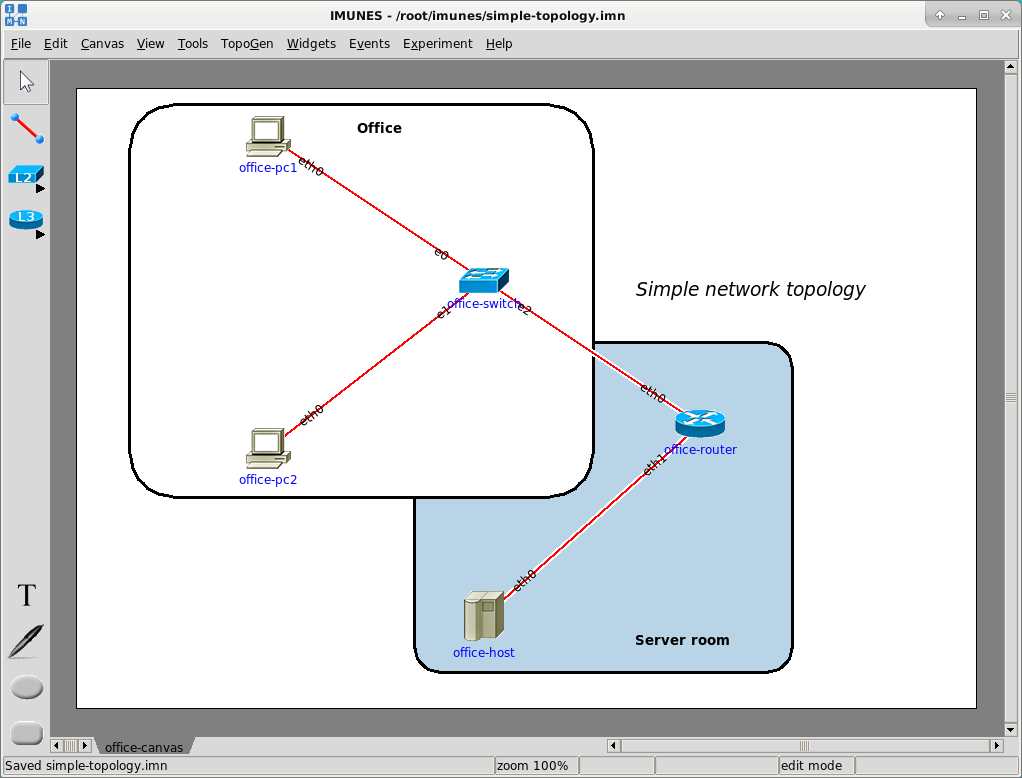
\includegraphics[width=\textwidth]{./images/topology_example.png}
\caption{\emph{Network topology}}
\label{fig:network_topology}
\end{figure} 

\begin{verbatim}
node n0 {
    type router
    model quagga
    network-config {
        hostname office-router
        !
        interface eth0
         mac address 42:00:aa:00:00:02
         ip address 192.168.1.1/24
        !
        interface eth1
         ipv6 address fc00:1::1/64
         mac address 42:00:aa:00:00:03
         ip address 192.168.2.1/24
        !
        interface lo0
         type lo
         ip address 127.0.0.1/8
         ipv6 address ::1/128
        !
        router rip
         redistribute static
         redistribute connected
         redistribute ospf
         network 0.0.0.0/0
        !
        router ripng
         redistribute static
         redistribute connected
         redistribute ospf6
         network ::/0
        !
    }
    canvas c0
    iconcoords {624 336}
    labelcoords {624 361}
    interface-peer {eth0 n2}
    interface-peer {eth1 n1}
}

node n1 {
    type host
    network-config {
        hostname office-host
        !
        interface eth0
         mac address 42:00:aa:00:00:04
         ip address 192.168.2.5/24
        !
        interface lo0
         type lo
         ip address 127.0.0.1/8
         ipv6 address ::1/128
        !
        ip route 0.0.0.0/0 192.168.2.1
        !
        !
    }
    canvas c0
    iconcoords {408 528}
    labelcoords {408 564}
    interface-peer {eth0 n0}
}

node n2 {
    type lanswitch
    network-config {
        hostname office-switch
        !
        interface e2
         fair-queue
        !
        interface e1
         fair-queue
        !
        interface e0
         fair-queue
        !
    }
    canvas c0
    iconcoords {408 192}
    labelcoords {408 215}
    interface-peer {e0 n3}
    interface-peer {e1 n4}
    interface-peer {e2 n0}
}

node n3 {
    type pc
    network-config {
        hostname office-pc1
        !
        interface lo0
         type lo
         ip address 127.0.0.1/8
         ipv6 address ::1/128
        !
        interface eth0
         mtu 1500
         mac address 42:00:aa:00:00:00
         ip address 192.168.1.5/24
        !
        !
        ip route 192.168.2.0/24 192.168.1.1
        !
    }
    canvas c0
    iconcoords {192 48}
    labelcoords {192 79}
    interface-peer {eth0 n2}
    custom-configs {
        custom-config-id newconf {
            custom-command /bin/sh
            config {
                ifconfig lo0 inet 127.0.0.1/8
                ifconfig eth0 inet 192.168.1.5/24
                ifconfig lo0 inet6 ::1
                
                route -q add -inet 192.168.2.0/24 192.168.1.1
                
                echo "Success!" > /tmp/log
                ifconfig vlan0
            }
        }
    }
    custom-enabled true
    custom-selected newconf
}

node n4 {
    type pc
    network-config {
        hostname office-pc2
        !
        interface eth0
         mac address 42:00:aa:00:00:01
         ip address 192.168.1.7/24
        !
        interface lo0
         type lo
         ip address 127.0.0.1/8
         ipv6 address ::1/128
        !
        ip route 192.168.2.0/24 192.168.1.1
        !
        !
    }
    canvas c0
    iconcoords {192 360}
    labelcoords {192 391}
    interface-peer {eth0 n2}
}

link l0 {
    nodes {n3 n2}
}

link l1 {
    nodes {n4 n2}
}

link l2 {
    delay 30000
    nodes {n2 n0}
    bandwidth 0
}

link l3 {
    nodes {n0 n1}
    bandwidth 0
}

annotation a0 {
    type rectangle
    iconcoords {53 16 517 409}
    color #ffffff
    bordercolor black
    width 3
    rad 53.6
    canvas c0
}

annotation a1 {
    type text
    iconcoords {281 40}
    label {Office}
    labelcolor #000000
    font {-family {DejaVu Sans} -size 10 -weight bold -slant roman -underline 0 -overstrike 0}
    canvas c0
}

annotation a2 {
    type rectangle
    iconcoords {338 254 716 584}
    color #b8d4e6
    bordercolor #000000
    width 3
    rad 30.78918918918919
    canvas c0
}

annotation a3 {
    type text
    iconcoords {559 552}
    label {Server room}
    labelcolor black
    font {-family {DejaVu Sans} -size 10 -weight bold -slant roman -underline 0 -overstrike 0}
    canvas c0
}

annotation a4 {
    type text
    iconcoords {560 201}
    label {Simple network topology}
    labelcolor black
    font {-family {DejaVu Sans} -size 14 -weight normal -slant italic -underline 0 -overstrike 0}
    canvas c0
}

canvas c0 {
    name {office-canvas}
}

option show {
    interface_names yes
    ip_addresses no
    ipv6_addresses no
    node_labels yes
    link_labels no
    background_images no
    annotations yes
    hostsAutoAssign no
    grid no
    iconSize normal
    zoom 1.0
}
\end{verbatim}
